\documentclass[sans,mathserif,aspectratio=169]{beamer}

\usepackage{booktabs}
\usepackage[spanish, mexico]{babel}
\selectlanguage{spanish}
\decimalpoint
\usepackage[utf8]{inputenc}
\usepackage{tikz}
\usepackage{fourier}
\newcommand{\quotes}[1]{``#1''}
\usepackage{epstopdf}
\usepackage{mathtools}
\DeclarePairedDelimiter{\ceil}{\lceil}{\rceil}
\usepackage{commath}
\usepackage{amsmath,tabularx}
\usepackage{listings}
\usepackage{xcolor}
\usepackage[edges]{forest}
\graphicspath{{Images/}}
\usepackage[mathscr]{euscript}
\newcommand{\overbar}[1]{\mkern 1.5mu\overline{\mkern-1.5mu#1\mkern-1.5mu}\mkern 1.5mu}
\newcommand*\mean[1]{\overbar{#1}}


\definecolor{foldercolor}{RGB}{124,166,198}

\tikzset{pics/folder/.style={code={%
    \node[inner sep=0pt, minimum size=#1](-foldericon){};
    \node[folder style, inner sep=0pt, minimum width=0.3*#1, minimum height=0.6*#1, above right, xshift=0.05*#1] at (-foldericon.west){};
    \node[folder style, inner sep=0pt, minimum size=#1] at (-foldericon.center){};}
    },
    pics/folder/.default={20pt},
    folder style/.style={draw=foldercolor!80!black,top color=foldercolor!40,bottom color=foldercolor}
}

\forestset{is file/.style={edge path'/.expanded={%
        ([xshift=\forestregister{folder indent}]!u.parent anchor) |- (.child anchor)},
        inner sep=1pt},
    this folder size/.style={edge path'/.expanded={%
        ([xshift=\forestregister{folder indent}]!u.parent anchor) |- (.child anchor) pic[solid]{folder=#1}}, inner xsep=0.6*#1},
    folder tree indent/.style={before computing xy={l=#1}},
    folder icons/.style={folder, this folder size=#1, folder tree indent=3*#1},
    folder icons/.default={12pt},
}

\colorlet{punct}{red!60!black}
\definecolor{background}{HTML}{EEEEEE}
\definecolor{delim}{RGB}{20,105,176}
\colorlet{numb}{magenta!60!black}

\lstdefinelanguage{json}{
    basicstyle=\normalfont\ttfamily\tiny,
    columns=flexible,
    keepspaces=true,
    frame=lines,
    backgroundcolor=\color{background}
}

\mode<presentation>

%Colors
\definecolor{steel}{RGB}{52,102,136}
\definecolor{moss}{RGB}{139,187,159}
\definecolor{burnt}{RGB}{187,102,65}
\definecolor{sandy}{RGB}{186, 168, 111}
\definecolor{RoyalBlue}{RGB}{0,35,102}
\definecolor{cream}{RGB}{254, 246, 235}
\definecolor{slate}{RGB}{82, 85, 100}
\definecolor{fall}{RGB}{194, 91, 86} % frame color
\definecolor{light}{RGB}{150, 192, 206}

%Structure
\usefonttheme{professionalfonts}
\hypersetup{colorlinks,linkcolor=fall!80,urlcolor=fall!80}
\setbeamercolor{local structure}{fg=fall}
\setbeamercolor{background canvas}{bg=cream}
\setbeamercolor{frametitle}{bg=fall,fg=cream}
\setbeamercolor{title}{fg=steel!115}
\setbeamercolor{author}{fg=fall}

\defbeamertemplate*{title page}{customized}[1][]
{\centering
  \fcolorbox{fall}{white}{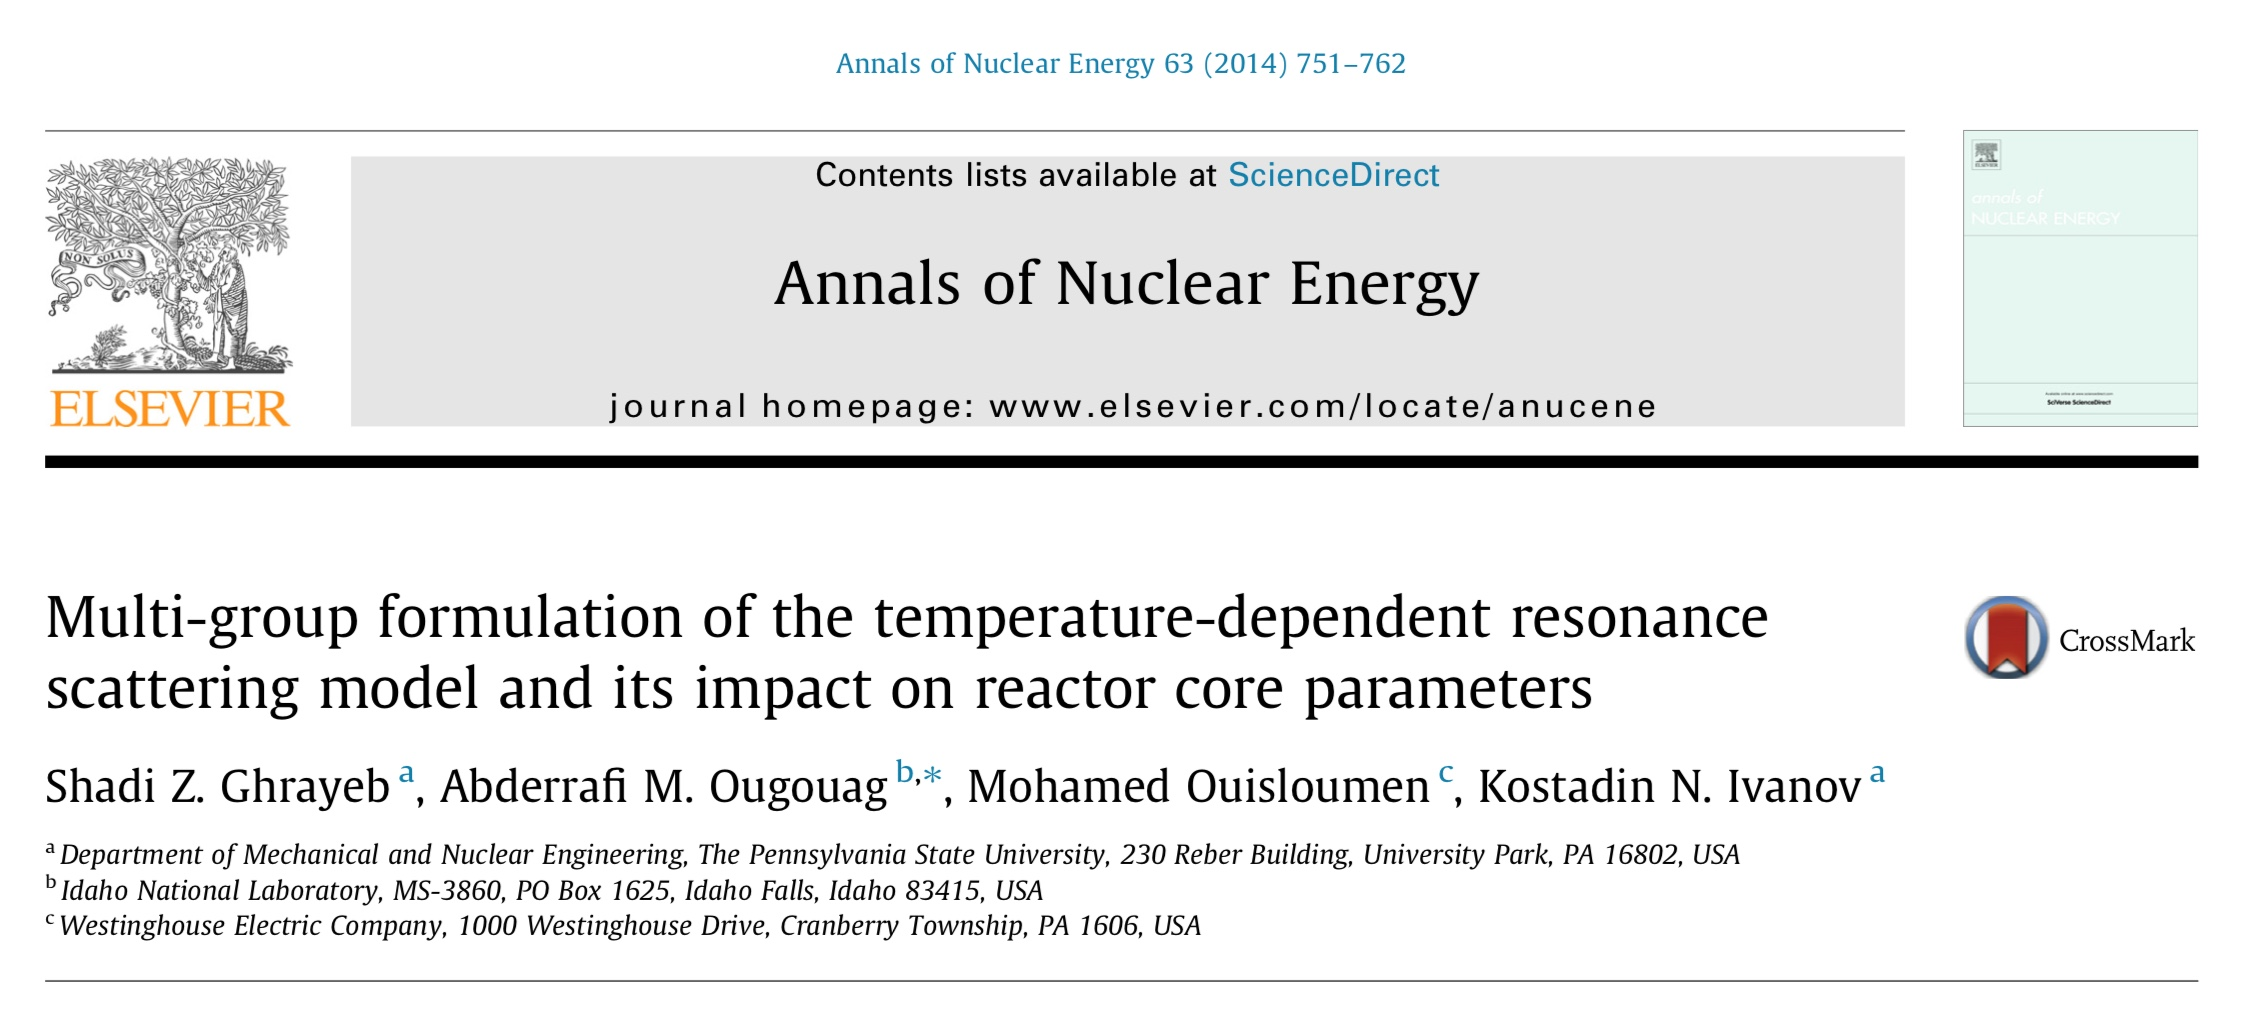
\includegraphics[width=0.80\linewidth]{cover.jpeg}}
  \vfill
  \usebeamerfont{author}\usebeamercolor[fg]{author}\insertauthor\par
  \vfill
  \usebeamerfont{institute}\insertinstitute\par
  \usebeamerfont{date}\insertdate\par
  \usebeamercolor[fg]{titlegraphic}\inserttitlegraphic
}

% Progressbar
\usepackage{tikz}
\usetikzlibrary{calc}

\makeatletter
\def\progressbar@progressbar{} % the progress bar
\newcount\progressbar@tmpcounta% auxiliary counter
\newcount\progressbar@tmpcountb% auxiliary counter
\newdimen\progressbar@pbht %progressbar height
\newdimen\progressbar@pbwd %progressbar width
\newdimen\progressbar@tmpdim % auxiliary dimension

\progressbar@pbwd=\paperwidth
\progressbar@pbht=2pt

\def\progressbar@progressbar{%

\progressbar@tmpcounta=\insertframenumber
\progressbar@tmpcountb=\inserttotalframenumber
\progressbar@tmpdim=\progressbar@pbwd
\multiply\progressbar@tmpdim by \progressbar@tmpcounta
\divide\progressbar@tmpdim by \progressbar@tmpcountb

  \begin{tikzpicture}[very thin]

  \shade[draw=steel!115,top color=steel,bottom color=steel,middle color=steel!115] %
    (0pt, 0pt) rectangle ++ (\progressbar@tmpdim, \progressbar@pbht);

  \end{tikzpicture}%
 }

\addtobeamertemplate{frametitle}{}
{%
  \vspace*{-16pt}
  \begin{beamercolorbox}[wd=\paperwidth,ht=1pt,dp=1pt]{}%
    \progressbar@progressbar%
  \end{beamercolorbox}%
}%
\makeatother

%Title
\title{Code Development Environment}
\subtitle{Experiences and Outlook}
\author[Guillermo Ibarra]{Guillermo Ibarra}
\date{Nuclear Engineering Research Seminar, March 24th, 2020}

\definecolor{keywords}{RGB}{255,0,90}
\definecolor{comments}{RGB}{0,0,113}
\definecolor{red}{RGB}{160,0,0}
\definecolor{green}{RGB}{0,150,0}

\setbeamercovered{transparent}
\setbeamercovered{%
  again covered={\opaqueness<1->{40}}}
\beamertemplatenavigationsymbolsempty


\begin{document}

%slide
\begin{frame}
\titlepage
\end{frame}

%slide
\begin{frame}{Slowing Down Equation}{Brief Introduction}
\begin{equation*}
\Sigma_t (E') \phi (E') = \int_0^\infty P (E \to E') \sigma_s (E) \phi (E) dE
\end{equation*}
\pause
\begin{align*}
\Sigma_t (E') \phi (E') &= \int_{E'}^{E'/\alpha} \frac{\sigma_s (E)}{(1-\alpha) E} \phi (E) dE \\
\sigma_s (E) P (E \to E') &= 
\begin{cases}
	\frac{\sigma_s (E)}{E (1 - \alpha)}, & \alpha E \le E' \le E,\\
	0, & otherwise.
\end{cases}
\end{align*}
\end{frame}

%slide
\begin{frame}{History of the Resonance Scattering Model}
\begin{itemize}
\item Ouisloumen and Sanchez (1990) - RSM
\item Rothenstein, 2004; Dagan, 2004 - $S(\alpha, \beta)$ tables
\item Becker et al. (2009b) - Doppler broadened rejection correction (DBRC) approach
\end{itemize}
\end{frame}

\begin{frame}{Summary of Results with the Mosteller Benchmark}
\centering
\fcolorbox{fall}{white}{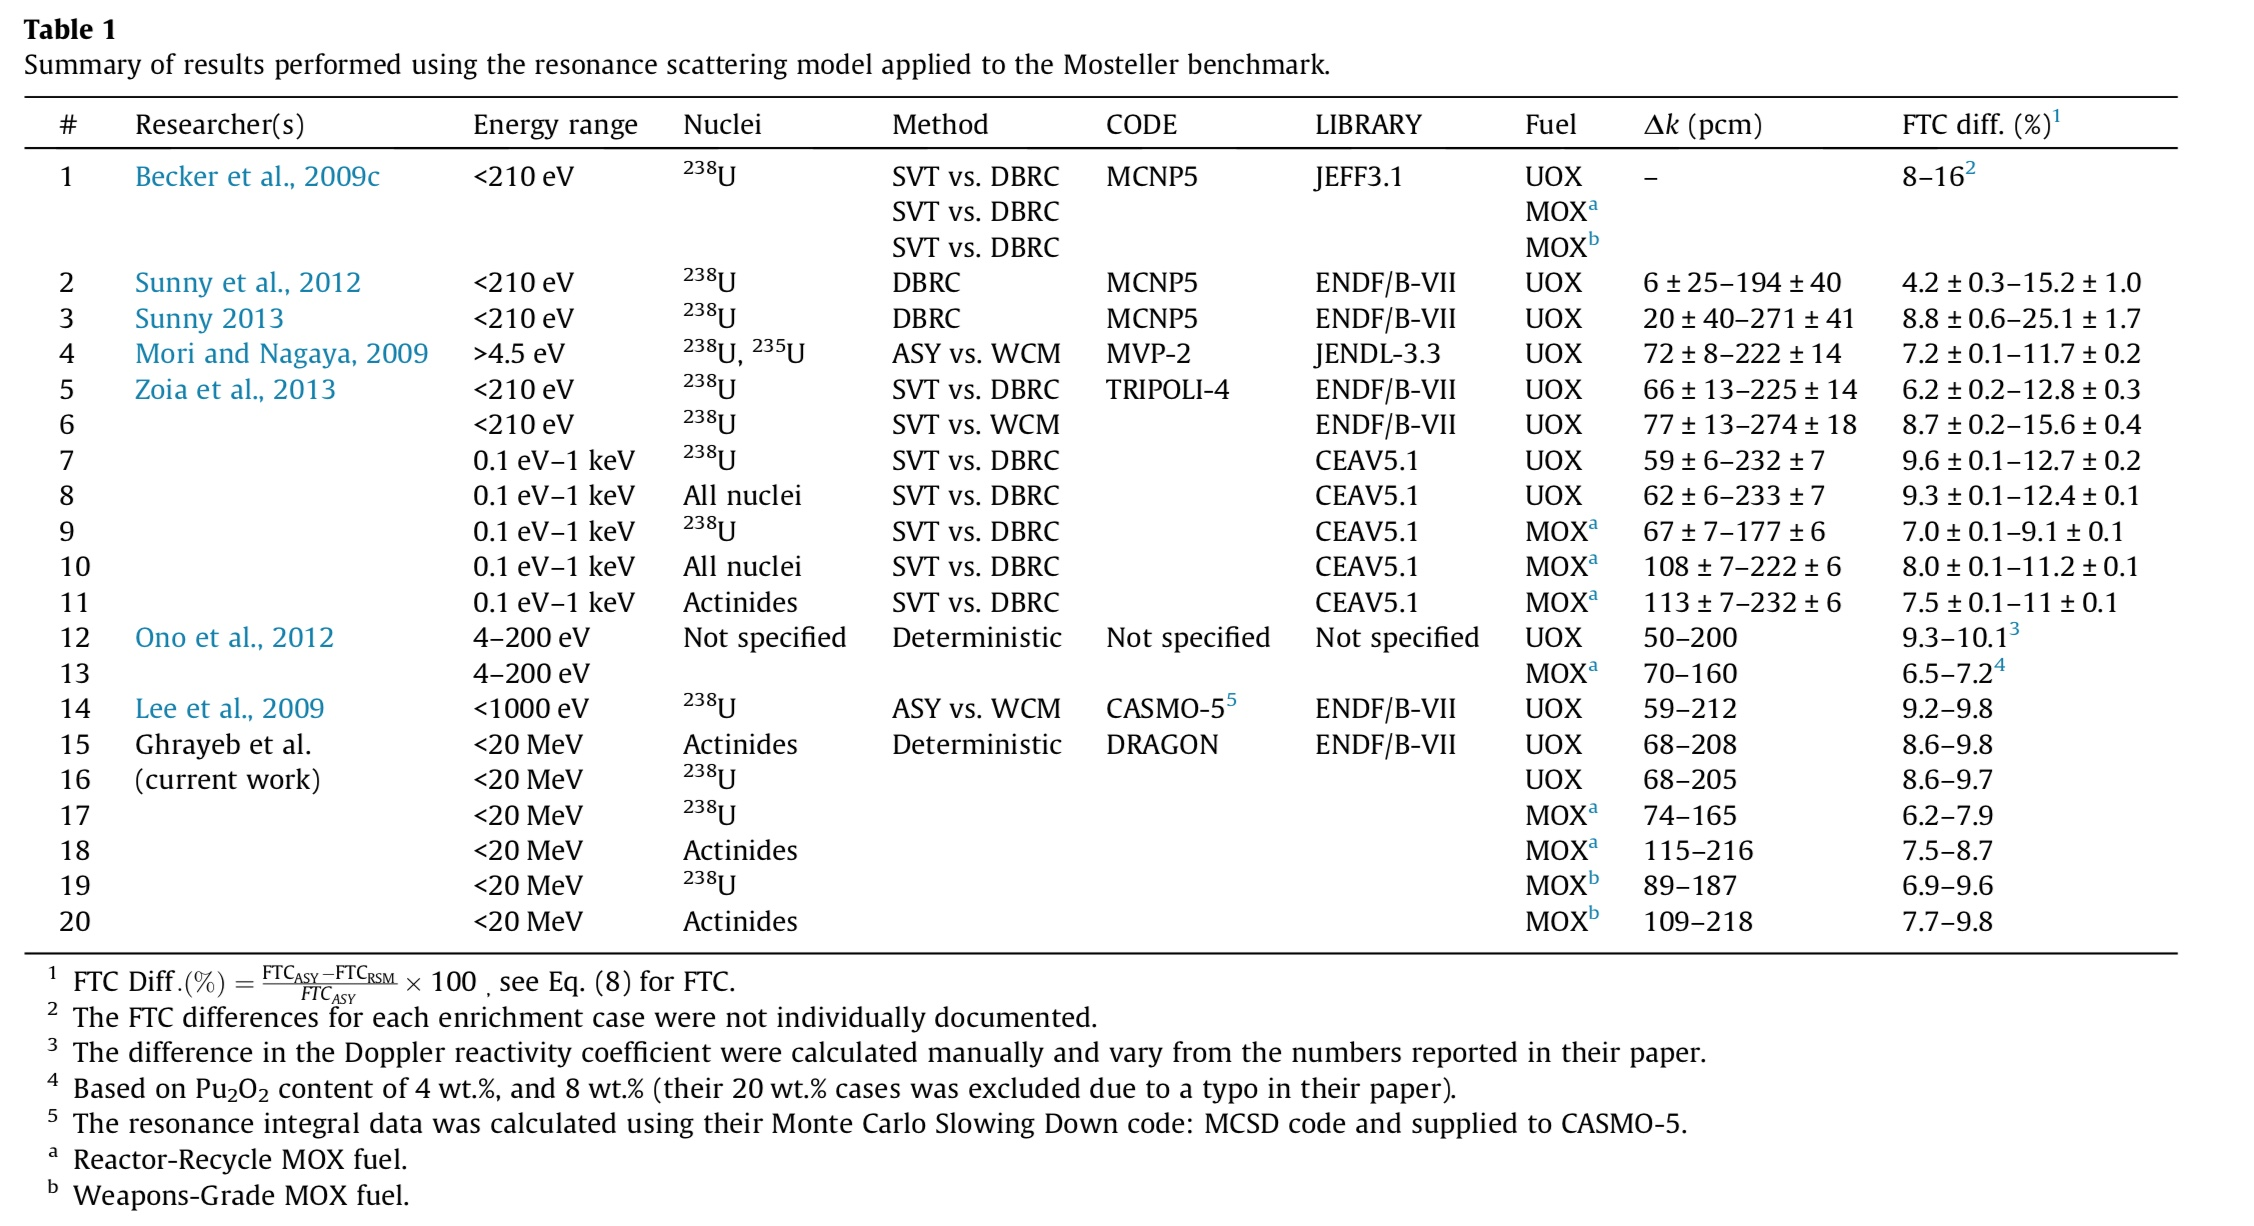
\includegraphics[width=0.90\linewidth]{table1.jpeg}}
\end{frame}

\begin{frame}{Formulation}
Ousilomen and Sanchez, 1990:
\begin{equation*}
\sigma_{sn}^T (E \to E') = \frac{\beta^{5/2}}{4E} e^{\frac{E}{kT}} \int_0^\infty t \sigma_s^{\text{tab}} \left( \frac{\beta k T}{A} t^2 \right)
e^{-\frac{t^2}{A}} \Psi_n (t) dt
\end{equation*}
\pause
For isotropic scattering:
\begin{equation*}
\sigma_{s_0, g \to g'}^T = \frac{1}{\delta_g \delta_g'} \int_{E_{g}}^{E_{g+1}} dE \int_{E_{g'}}^{E_{g'+1}} dE' \sigma_{s_0}^T (E \to E')
\end{equation*}
\pause
For within group scattering:
\begin{equation*}
\sigma_{s_0, g \to g'}^T = \frac{1}{\delta_g \delta_g} \int_{E_{g}}^{E_{g+1}} dE \left\{  \int_{E_{g}}^{E} dE' \sigma_{s_0}^T (E \to E') + \int_{E}^{E_{g+1}} dE' \sigma_{s_0}^T (E \to E') \right\}
\end{equation*}
\end{frame}

%slide
\begin{frame}{Test Implementation}
Multi-group implementation of the scattering kernel with $\delta_g < 10^{-3} eV$
\begin{align*}
&\delta_g \to 0, \delta_{g'} \to 0 \Rightarrow \sigma_{s_0, t \to g'}^T \approx \sigma_{s_0}^T (\mean{E}_g \to \mean{E}_{g'}); \\
& \mean{E}_g,  \mean{E}_{g'} = \frac{E_{g+1} + E_g}{2}, \frac{E_{g'+1} + E_{g'}}{2}
\end{align*}
\end{frame}

%slide
\begin{frame}{Scattering kernel of $^{238}$U at 1000 K }
\centering
\fcolorbox{fall}{white}{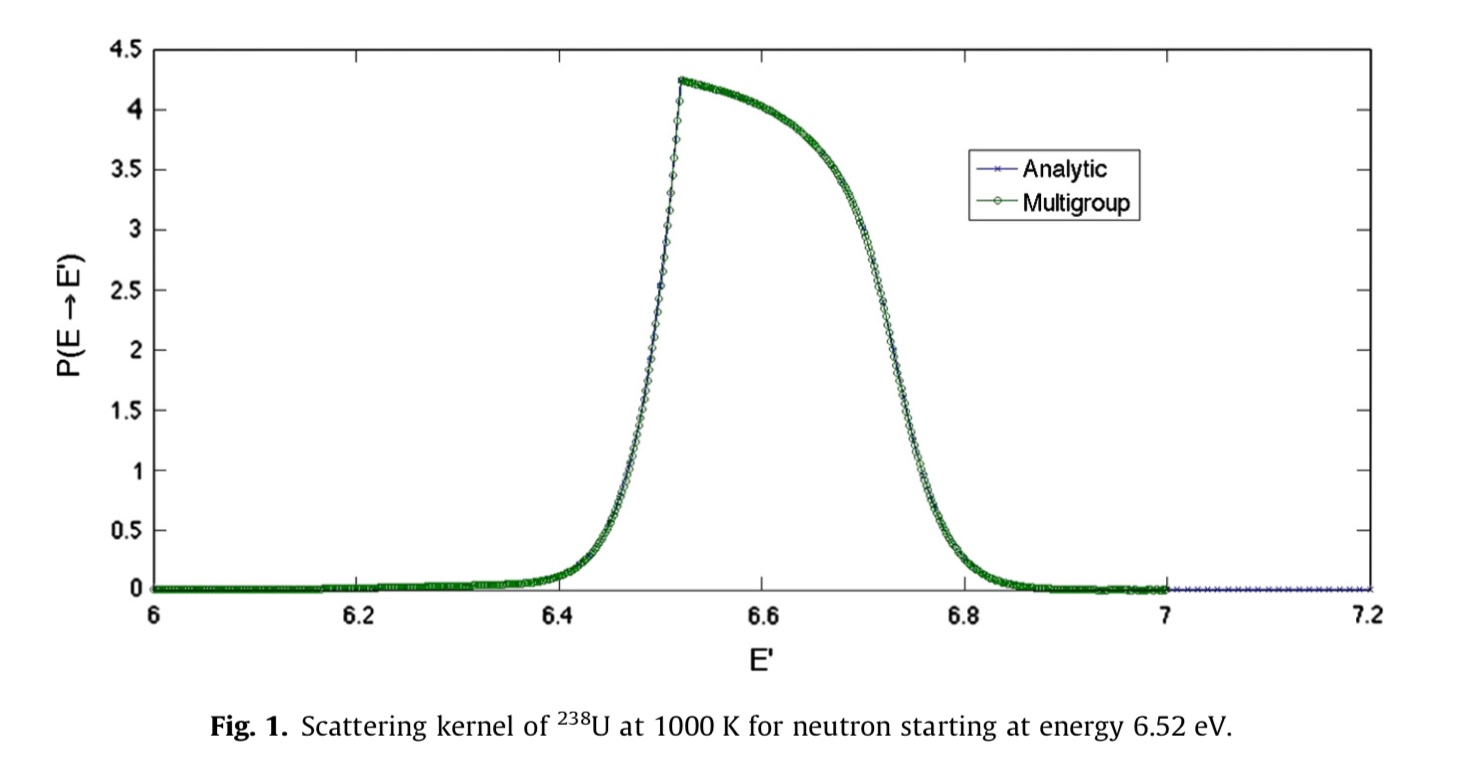
\includegraphics[width=0.50\linewidth]{fig1.jpeg}}
\fcolorbox{fall}{white}{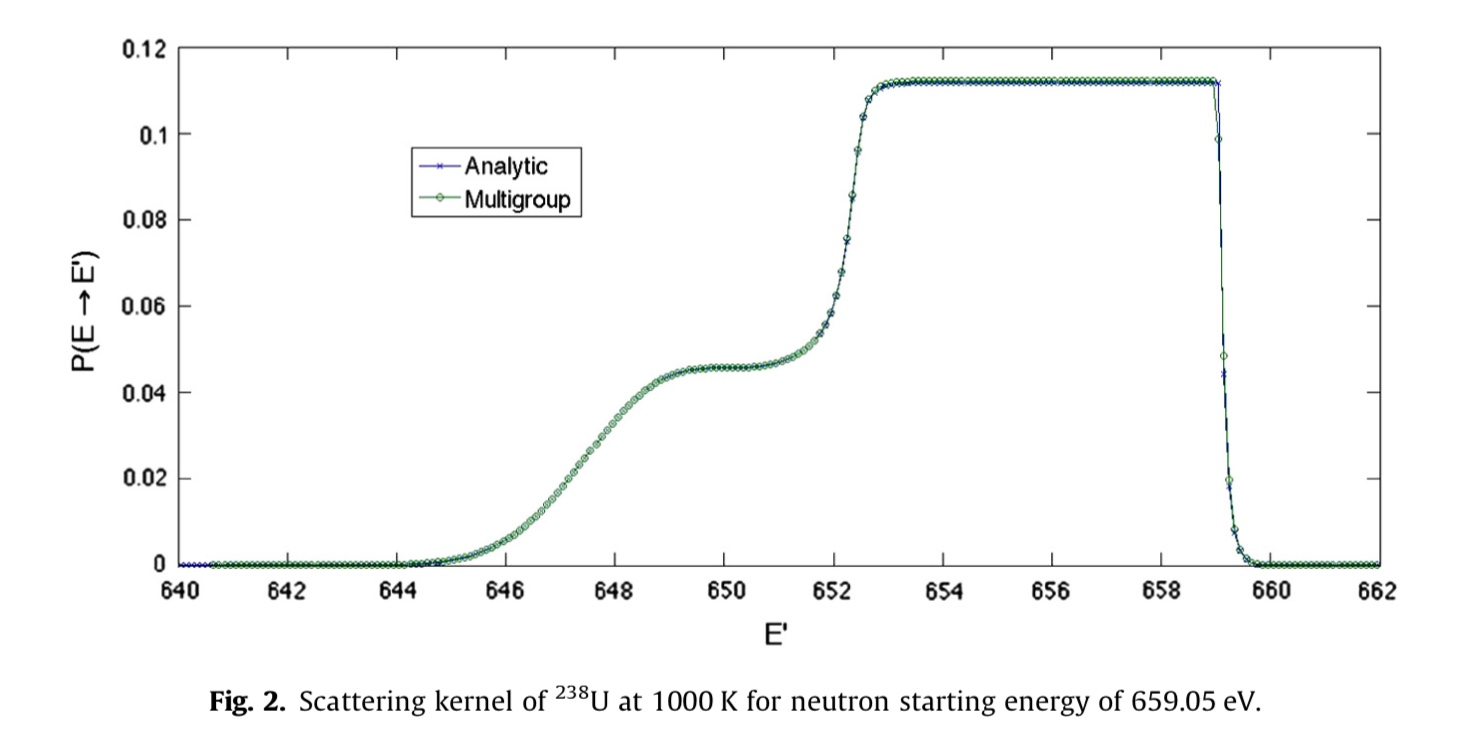
\includegraphics[width=0.50\linewidth]{fig2.jpeg}}
\end{frame}

%slide
\begin{frame}{Comparison with NJOY}
\centering
\fcolorbox{fall}{white}{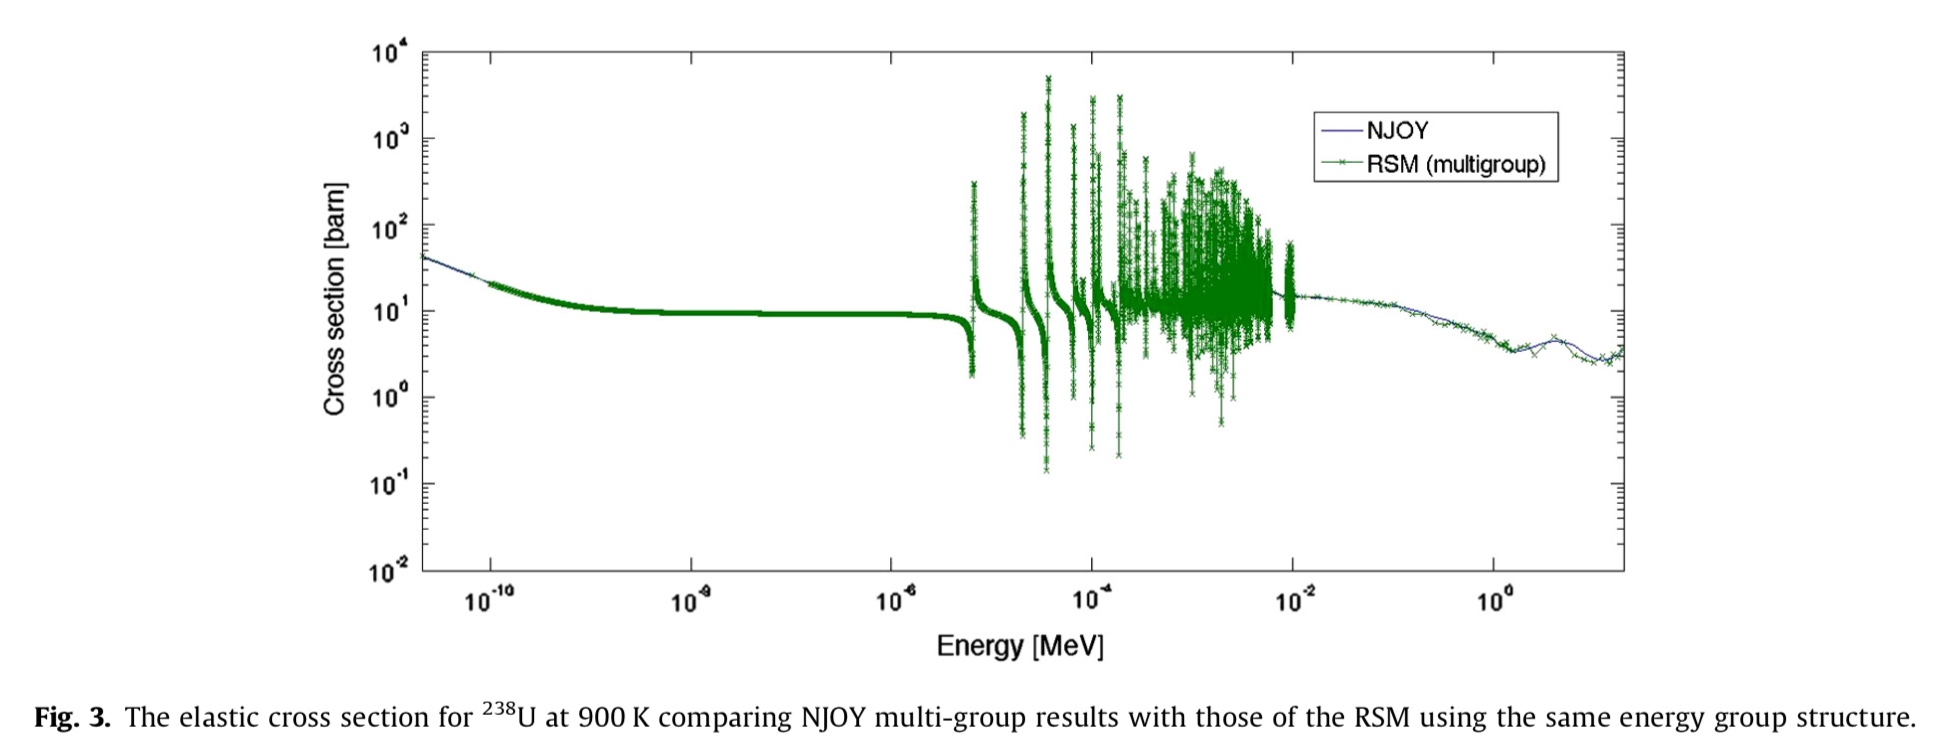
\includegraphics[width=0.90\linewidth]{fig3.jpeg}}
\end{frame}

%slide
\begin{frame}{Multi-group RSM with Mosteller Benchmark}
\begin{itemize}
\item Using DRAGON Code, Marleau et al., 2010 \pause
\item Scattering matrices generated with RSM calculation combined with NJOY data \pause
\item Fuel temperature coefficient:
\begin{equation*}
FTC = \left(\frac{1}{k_{HZP}} - \frac{1}{k_{HFP}} \right) \frac{1\times 10^5}{\Delta T}
\end{equation*}
\end{itemize}
\end{frame}

\begin{frame}{Mosteller UOX benchmark, RSM kernel applied only to $^{238}$U}
\centering
\fcolorbox{fall}{white}{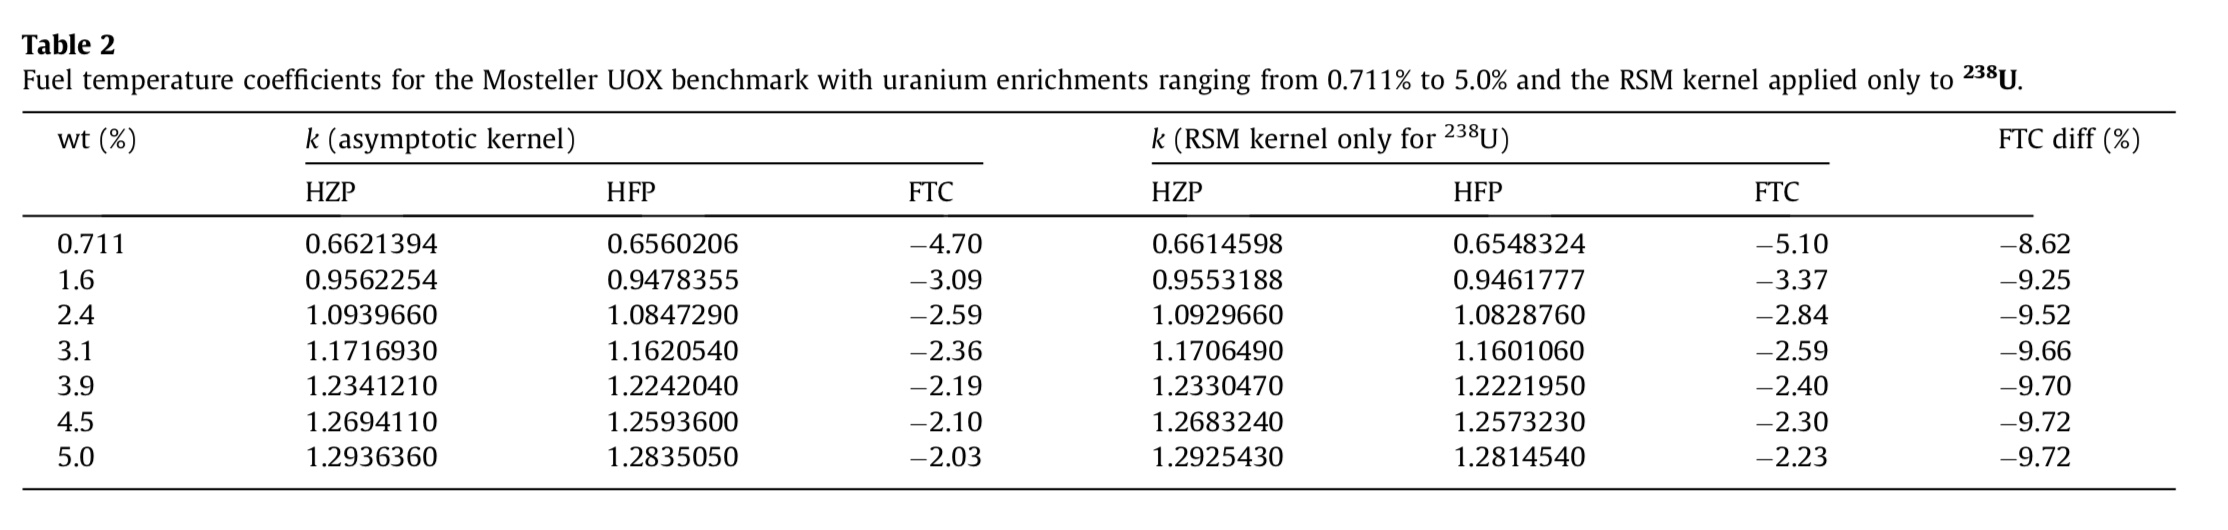
\includegraphics[width=\linewidth]{table2.jpeg}}
\end{frame}

\begin{frame}{Mosteller UOX benchmark, RSM kernel applied to all heavy nuclides}
\centering
\fcolorbox{fall}{white}{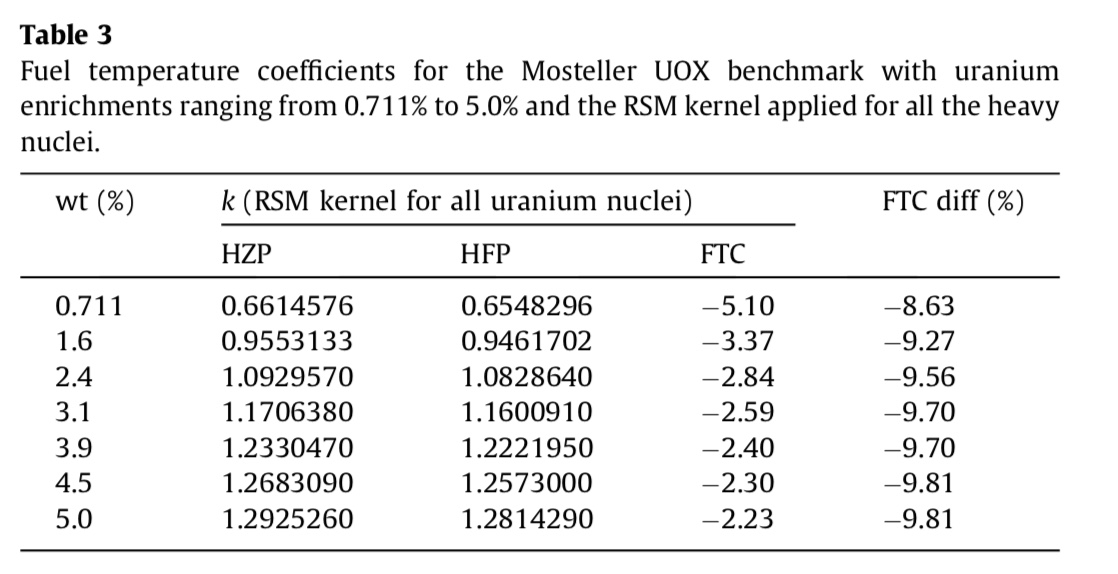
\includegraphics[width=0.9\linewidth]{table3.jpeg}}
\end{frame}

%slide
\begin{frame}{FTCs, RSM kernel applied to all heavy nuclides}
\centering
\fcolorbox{fall}{white}{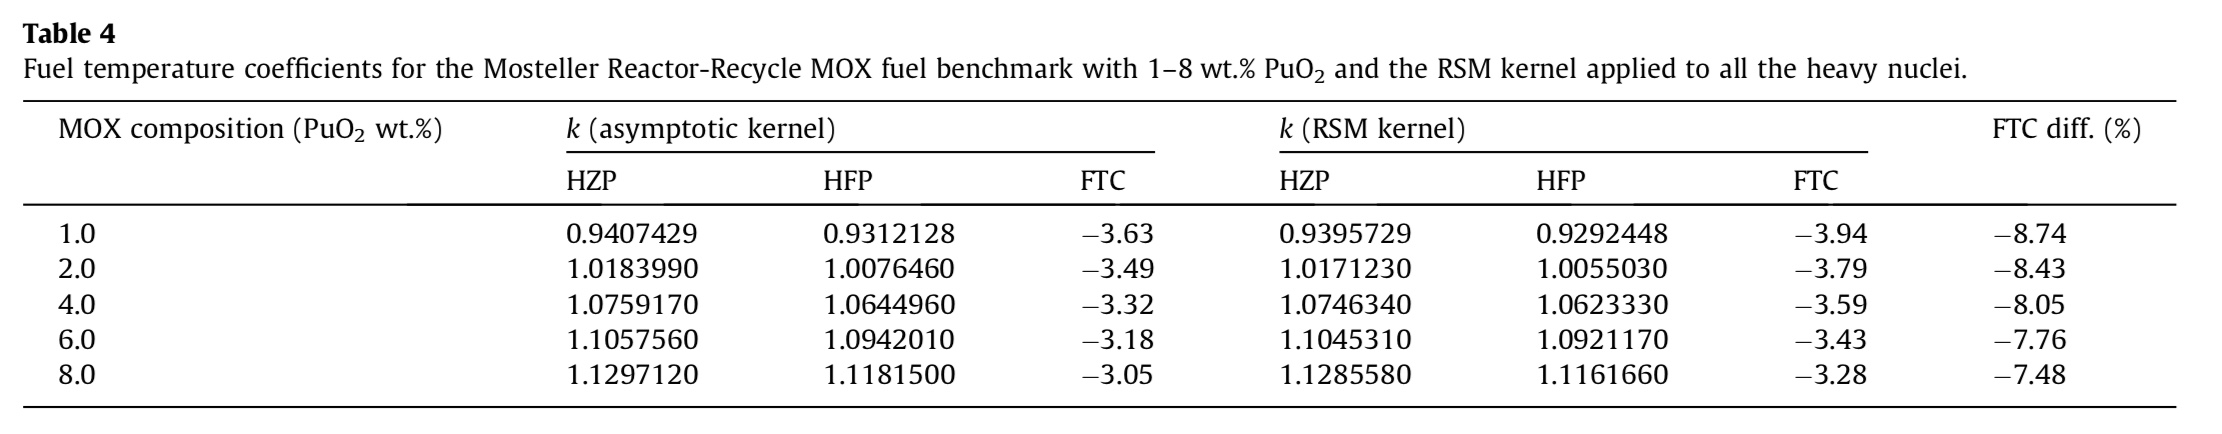
\includegraphics[width=\linewidth]{table4.jpeg}}
\fcolorbox{fall}{white}{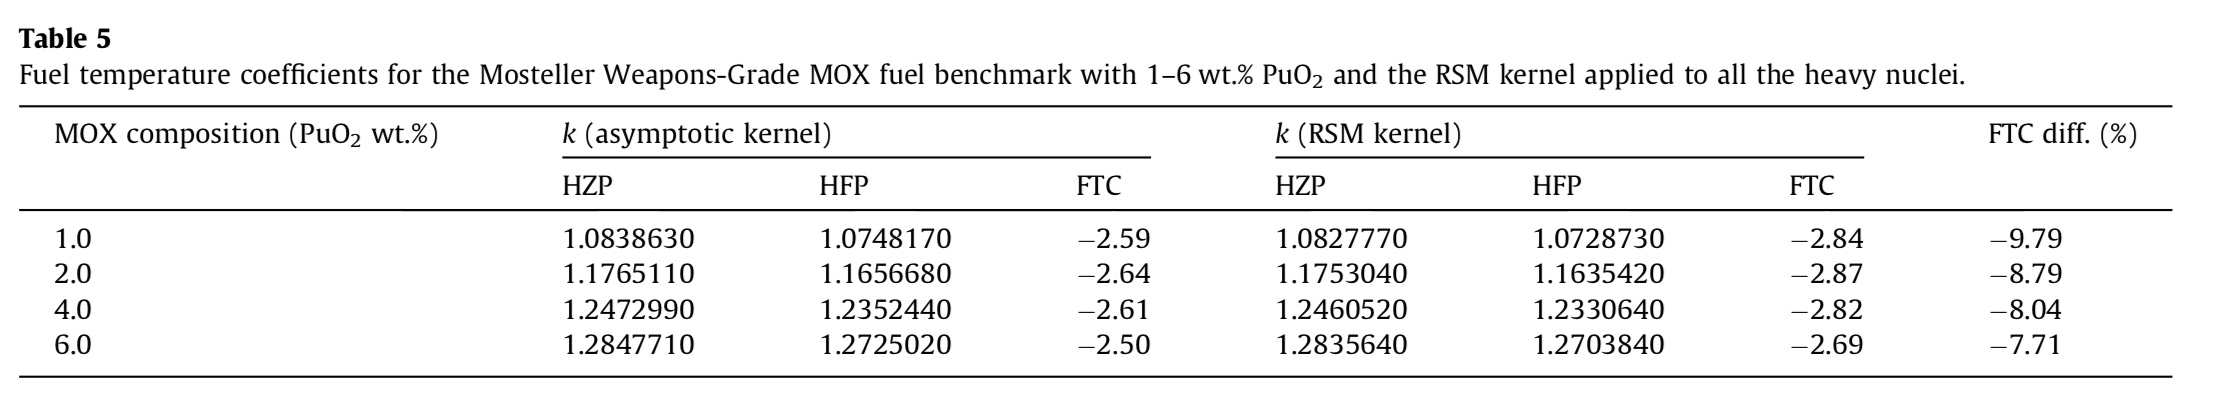
\includegraphics[width=\linewidth]{table5.jpeg}}
\end{frame}

%slide
\begin{frame}{FTCs, RSM kernel applied only to $^{238}$U}
\centering
\fcolorbox{fall}{white}{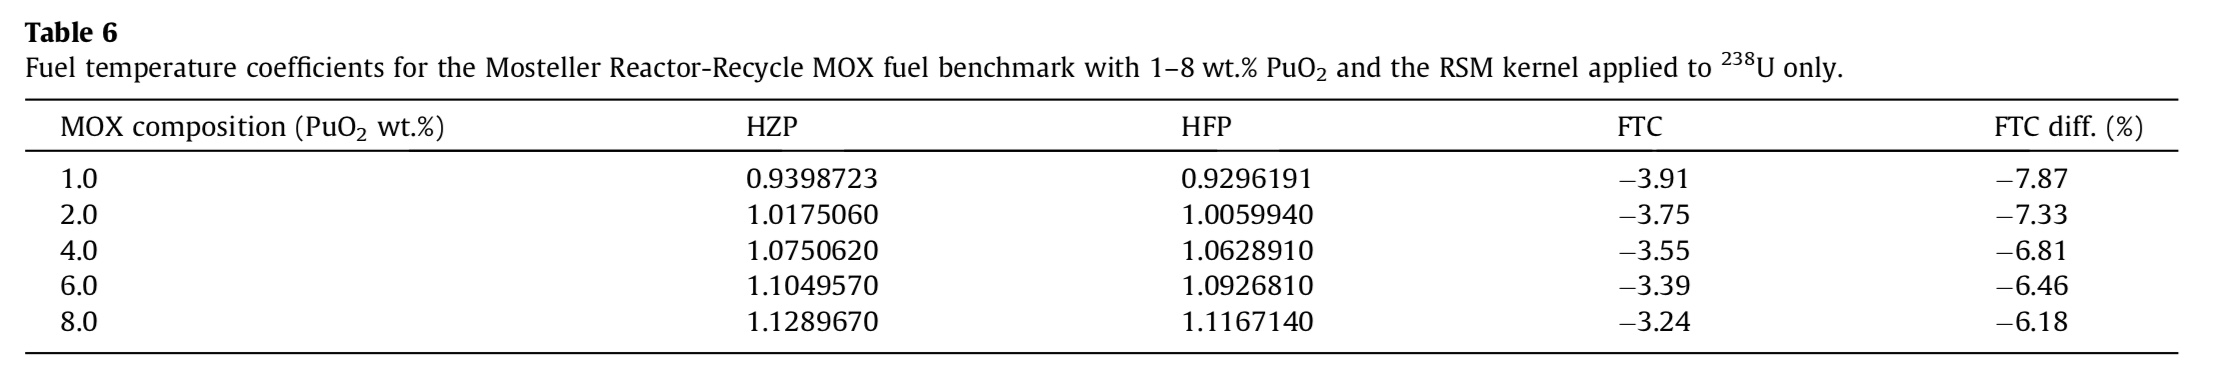
\includegraphics[width=\linewidth]{table6.jpeg}}
\fcolorbox{fall}{white}{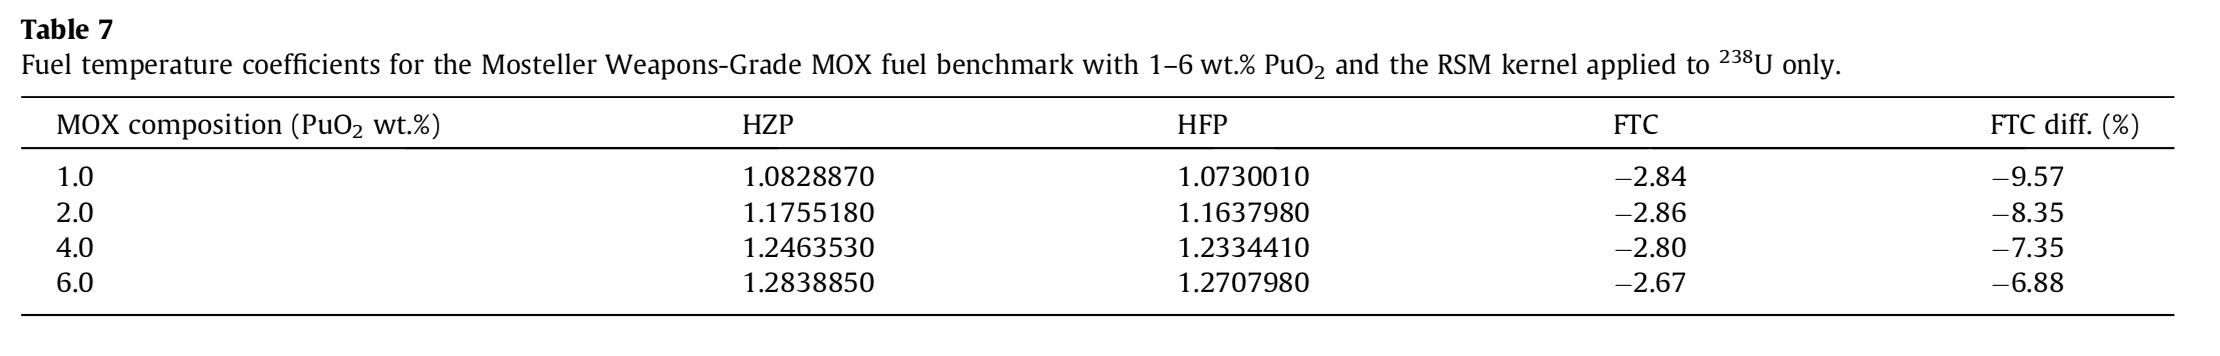
\includegraphics[width=\linewidth]{table7.jpeg}}
\end{frame}

%slide
\begin{frame}{FTCs, RSM kernel applied to individual nuclei}
\centering
\fcolorbox{fall}{white}{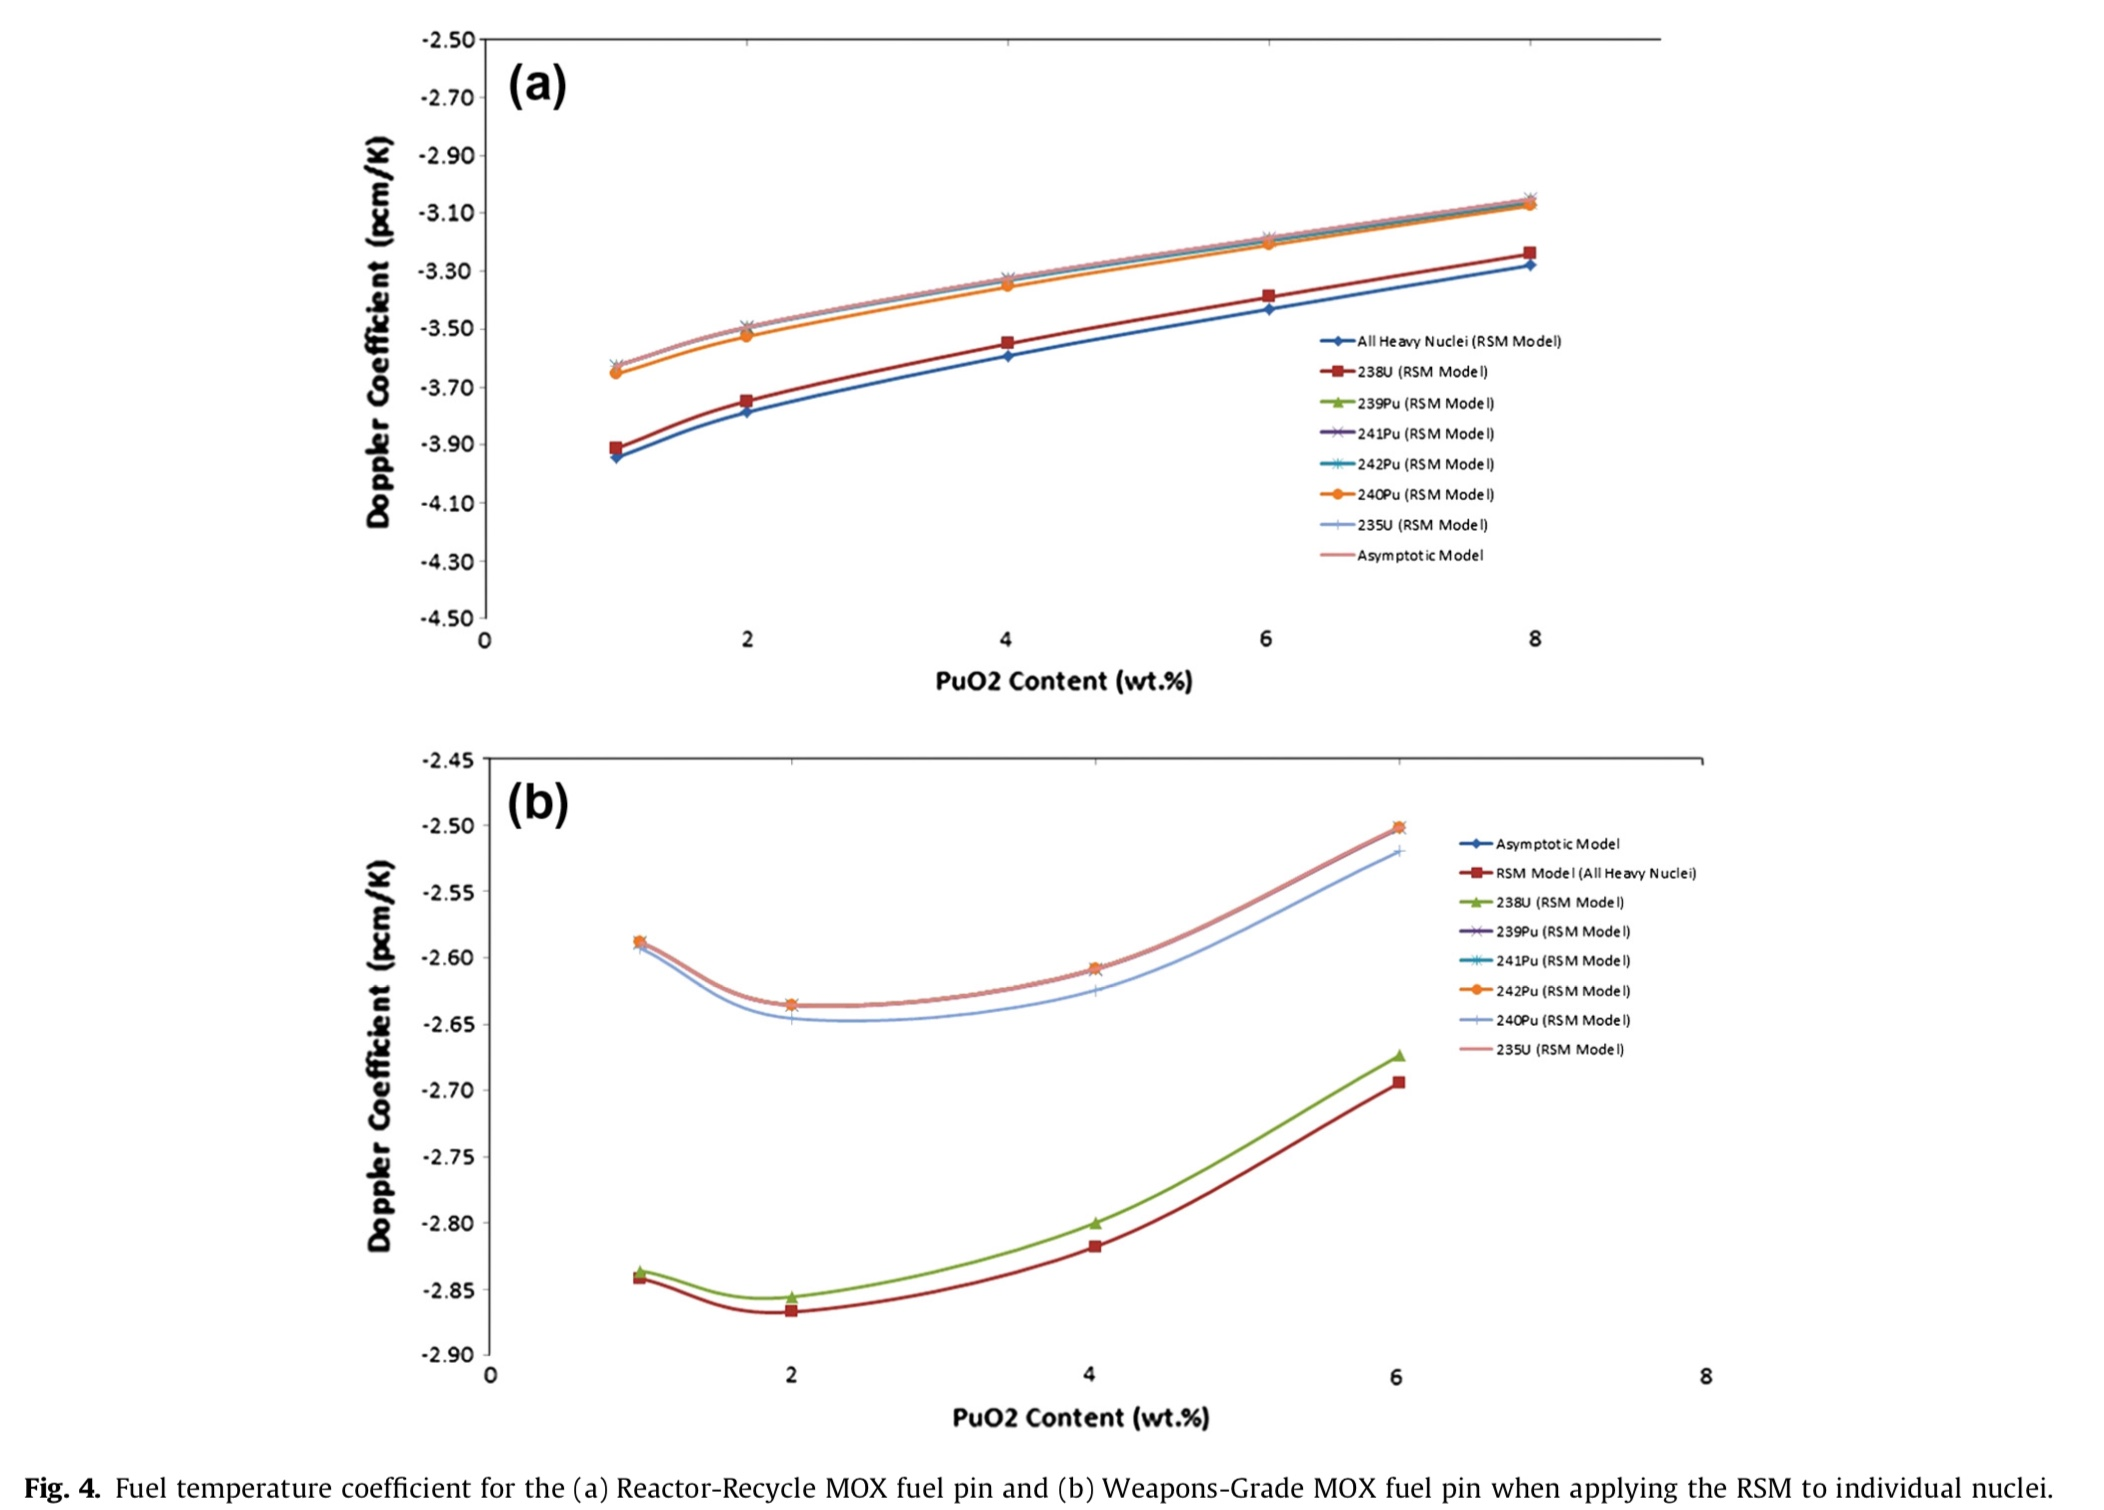
\includegraphics[width=0.65\linewidth]{fig4.jpeg}}
\end{frame}

\begin{frame}{Mini}
\begin{minipage}{0.48\linewidth}
\fcolorbox{fall}{white}{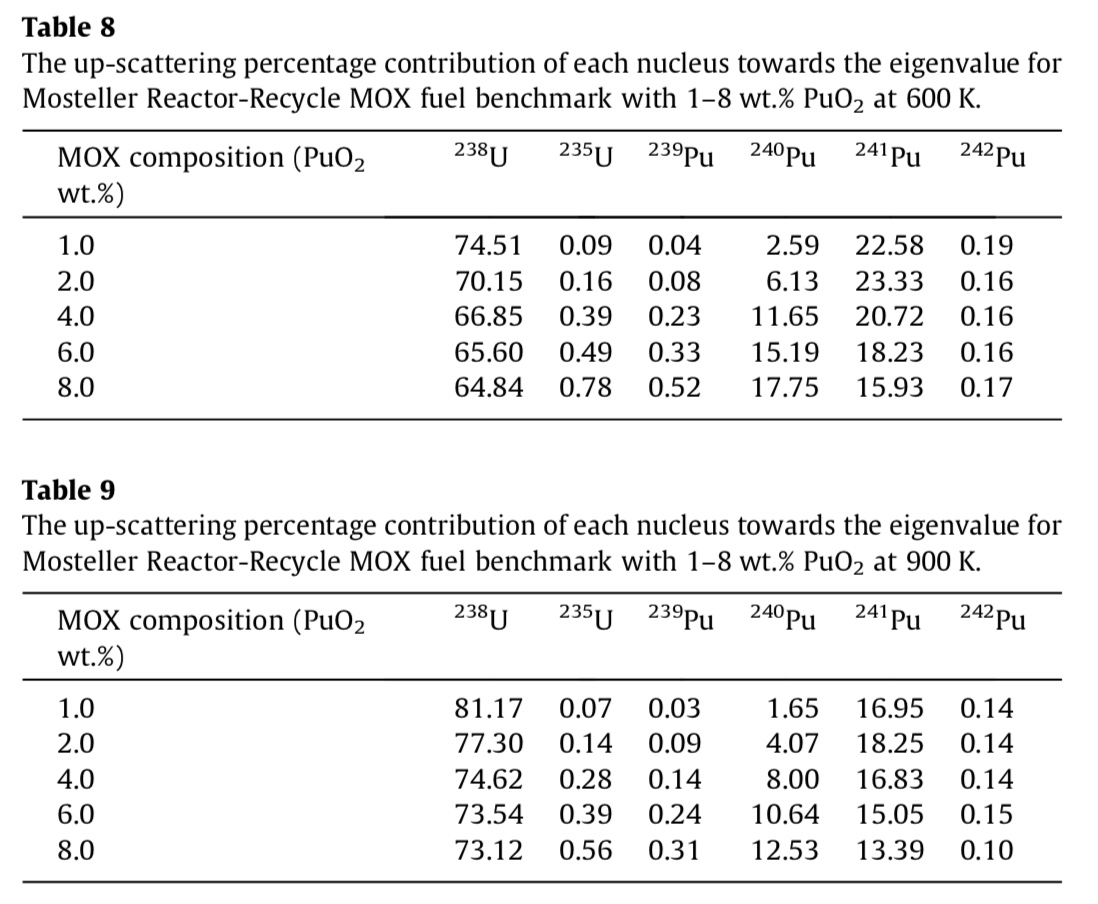
\includegraphics[width=\linewidth]{table8-9.jpeg}}
\end{minipage}\hfill
\begin{minipage}{0.48\linewidth}
\fcolorbox{fall}{white}{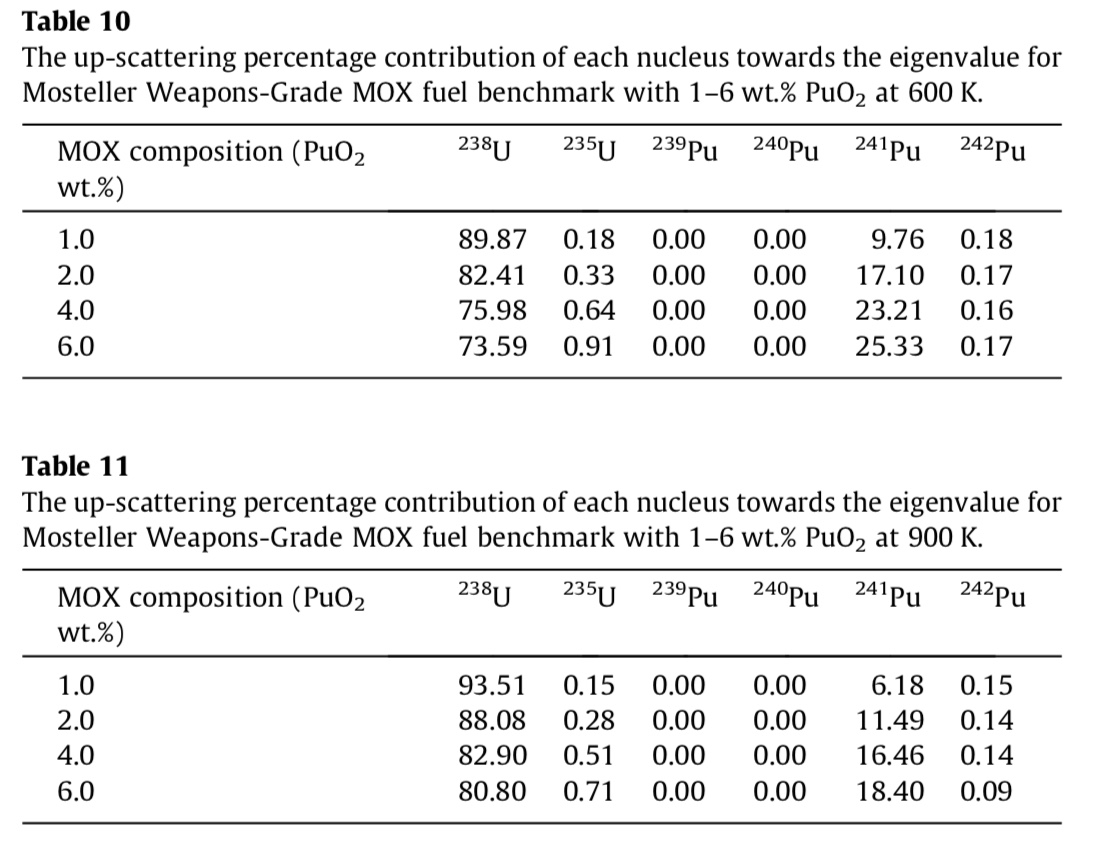
\includegraphics[width=\linewidth]{table10-11.jpeg}}
\end{minipage}
\end{frame}

%slide
\begin{frame}{Neutron Flux Near Third Resonance of $^{238}$U}
\centering
\fcolorbox{fall}{white}{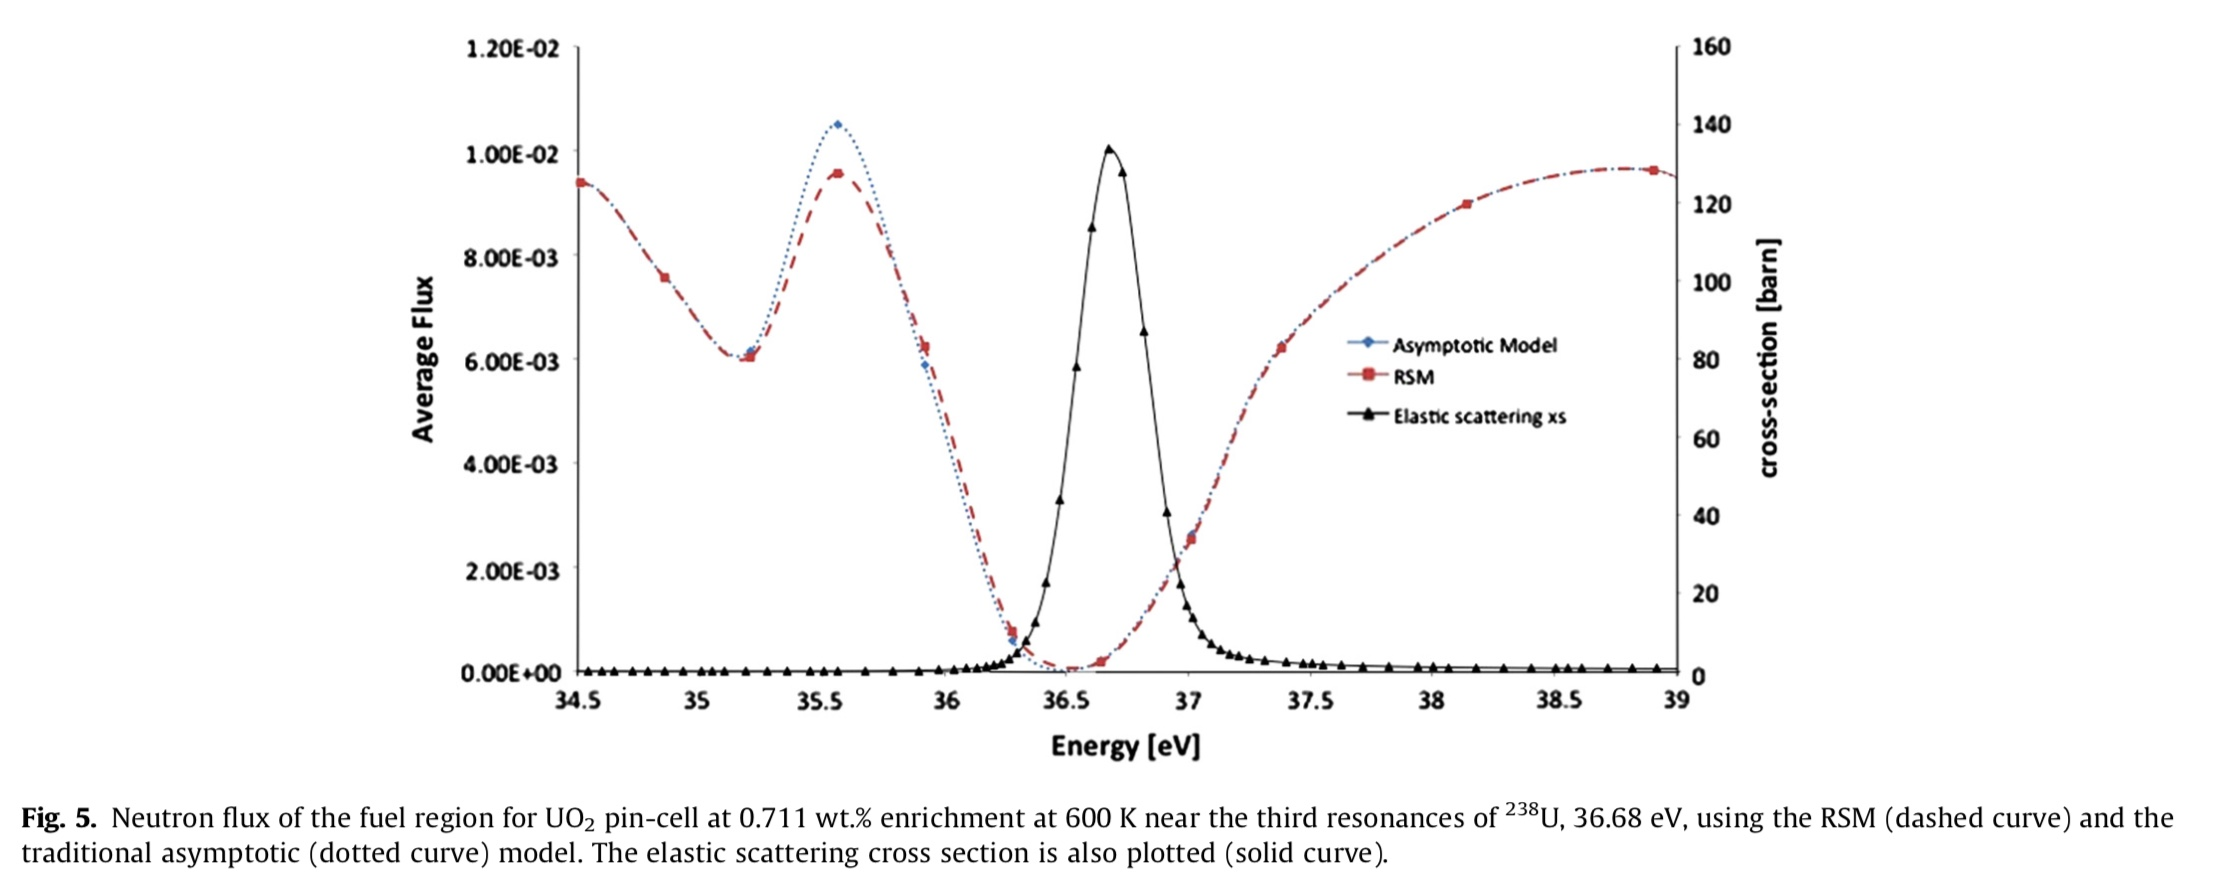
\includegraphics[width=\linewidth]{fig5.jpeg}}
\end{frame}

%slide
\begin{frame}{Relative Differences}
\centering
\fcolorbox{fall}{white}{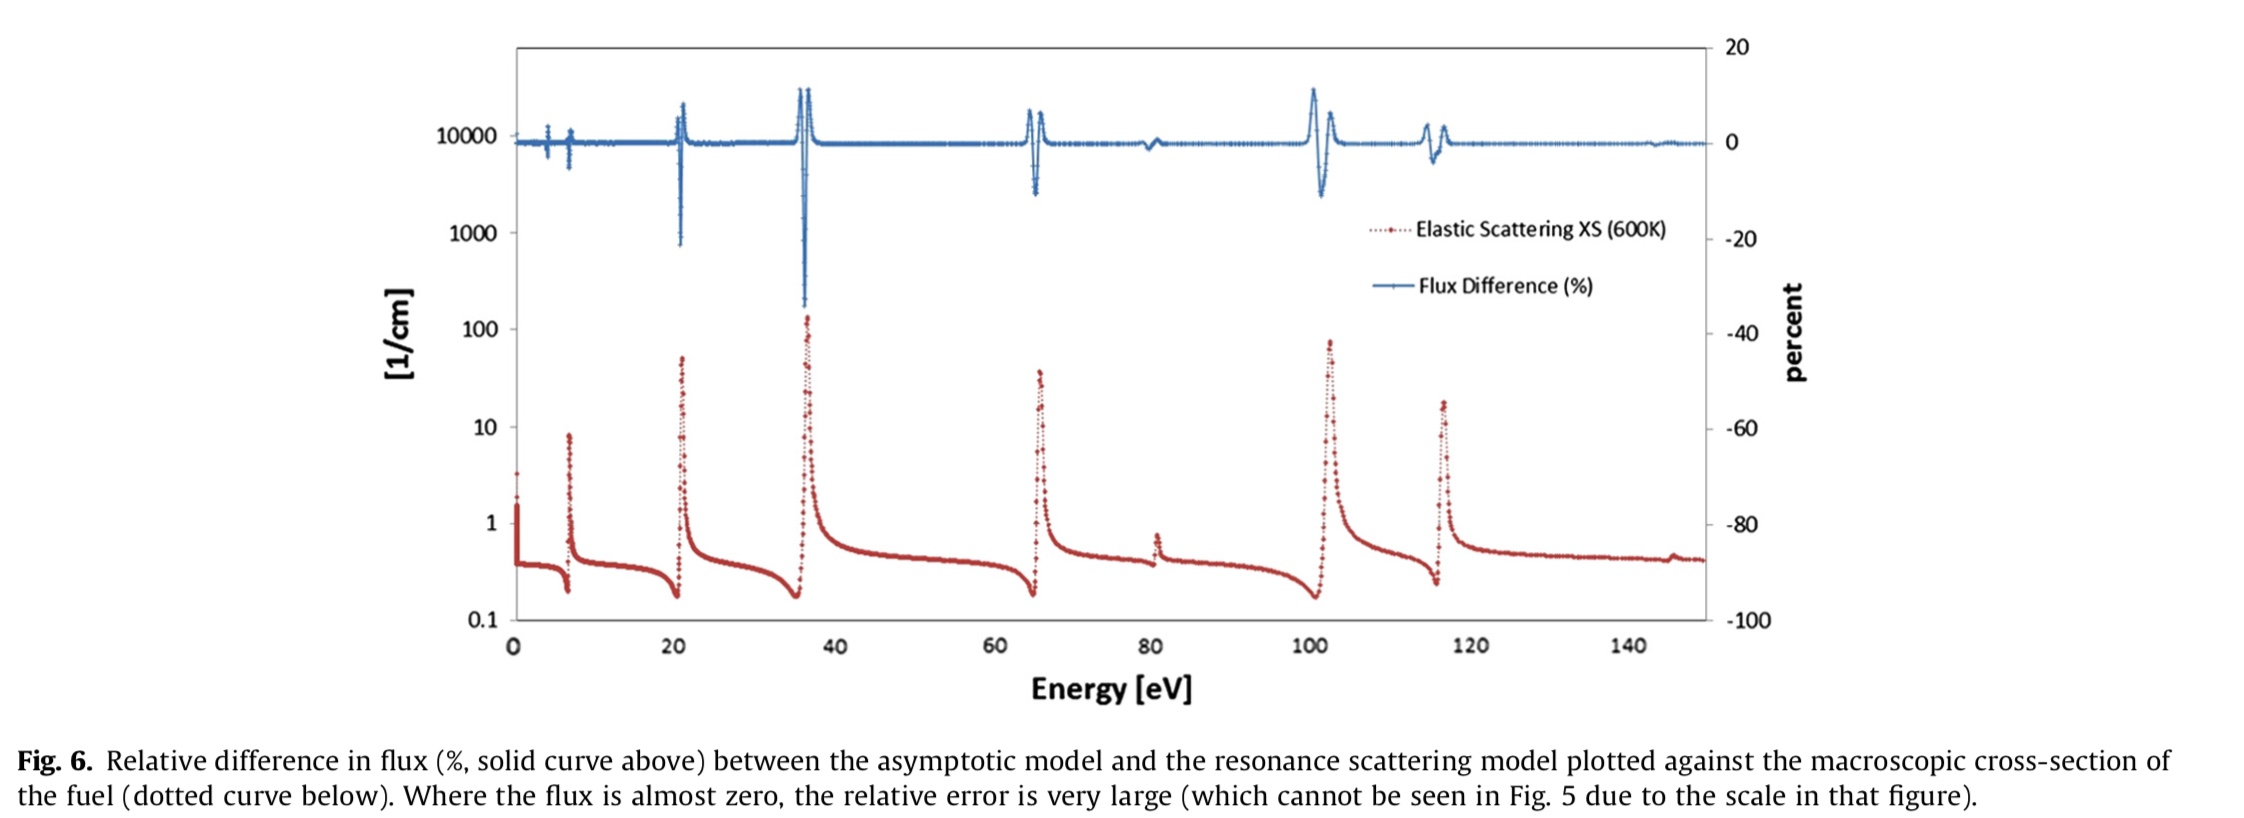
\includegraphics[width=\linewidth]{fig6.jpeg}}
\end{frame}

%slide
\begin{frame}{Comparison of Works with the Mosteller Benchmark}
\centering
\fcolorbox{fall}{white}{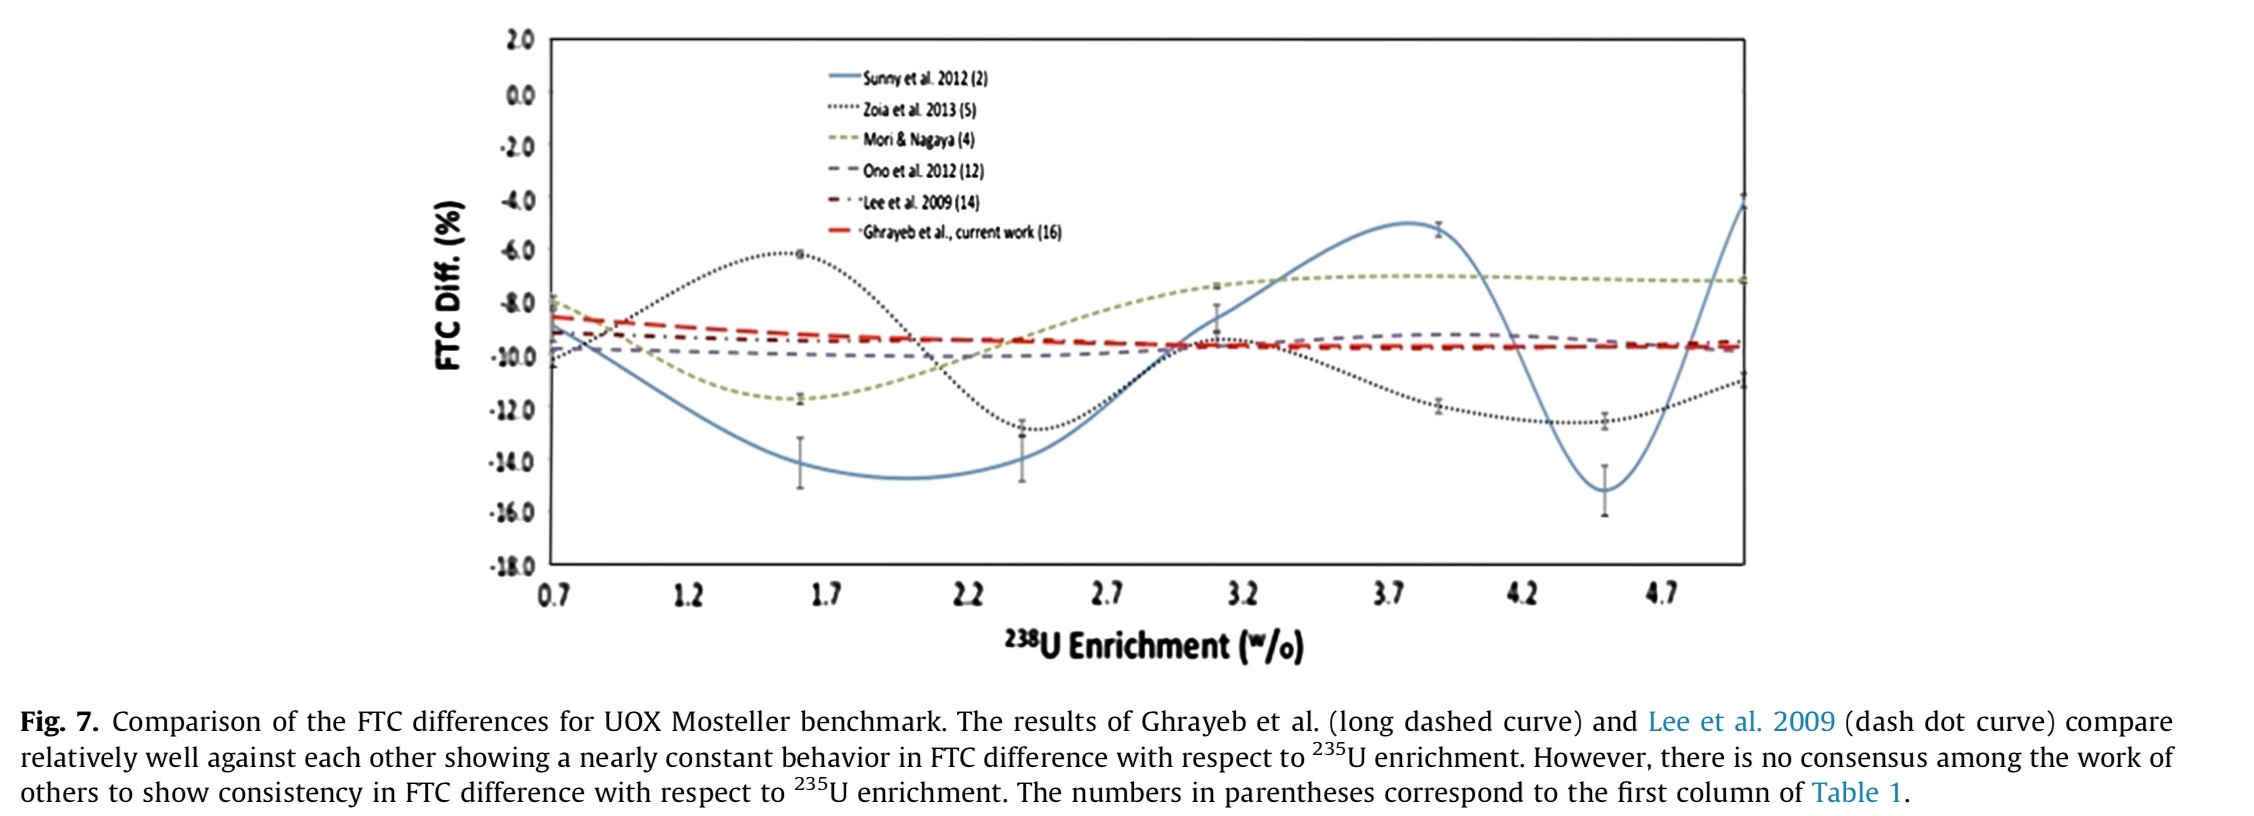
\includegraphics[width=\linewidth]{fig7.jpeg}}
\end{frame}

%slide
\begin{frame}{Summary of Main Aspects, TLDR}
\begin{itemize}
\item Temperature-dependent resonance scattering and up scattering effects are considered in slowing down calculation. \pause
\item Asymptotic model for neutron-nuclei elastic scattering under predicts the Doople coefficient by as much as 10\% in LWR lattices. \pause
\item In the case of the UO$_2$ fuel, the contribution of up-scattering was overwhelmingly due to $^{238}$U. \pause
\item When using RSM instead of asymptotic model, in case of UO$_2$ fuel, change in eigenvalues varies from 68 to 208 pcm.\pause
\item In the case of the weapons-grade MOX fuel the largest and most significant contribution to resonance up-scattering after that of $^{238}$U is that of $^{241}$Pu, which is responsible for as much as 25\% of up-scattering
\end{itemize}
\end{frame}

%slide
\begin{frame}
\centering
\Huge
Thanks! \\
Questions?
\end{frame}


\end{document}
